\section{手征对称性}

量子色动力学的拉氏量除了拥有$SU(3)_{color}$和$SU(3)_{flavor}$近似对称性以外还存在着另外一种对称性——手征对称性

当动量转移$Q \sim 1 {\rm~GeV/c}$的时候三种最轻的夸克,上、下和奇异夸克可以被近似地认为质量为零。在这种情况下拉氏量可以被写为:
\begin{equation}
    \label{QCDLagrangian}
    \mathcal{L} = i\bar{\phi}_f \gamma^{\mu} \delta_{\mu} \phi_{f}
\end{equation}

其中f表示夸克的味道。此拉氏量的一个重要的性质是在矢量和轴矢量变换下都有对称性:

\begin{equation}
    \label{Vector}
    \phi \rightarrow e^{i \alpha^{a}_{V}\frac{\lambda_a}{2}} \phi
\end{equation}
\begin{equation}
    \label{AxialVector}
    \phi \rightarrow e^{i \gamma_5 \alpha^{a}_{A}\frac{\lambda_a}{2}} \phi
\end{equation}

矢量和轴矢量的波函数可以用他们的左手或者右手手征分量来表示:

\begin{equation}
    \phi_{R,L} = \frac{1}{2}(1 \pm \gamma_5) \phi
\end{equation}

当我们考虑手征分量的时候变换\ref{Vector}和\ref{AxialVector}可以表示为:

\begin{equation}
    \phi_R \rightarrow e^{i \gamma_5 \alpha^{a}_{R}\frac{\lambda_a}{2}} \phi_R~,~\phi_L \rightarrow \phi_L
\end{equation}
\begin{equation}
    \phi_L \rightarrow e^{i \gamma_5 \alpha^{a}_{L}\frac{\lambda_a}{2}} \phi_L~,~\phi_R \rightarrow \phi_R
\end{equation}

在矢量和轴矢量的变化下我们可以看到一个由手征分量构成的对称性,这种在夸克质量为零的条件下的$SU(N_f)_{R} \times SU(N_f)_{L}$对称性被称作手征对称性。

当夸克质量不为零的时候其可以为视为量子色动力学拉氏量\ref{QCDLagrangian}当中的一个微扰项($\delta\mathcal{L} = -m\bar{\phi}\phi$)。这个微扰项带来了在轴矢量变换下的对称性破缺,因此也打破了手征对称性。对称性破缺可以表现为显式的对称性破缺或者是自发对称破缺。在显式对称性破缺中,对称性的破缺表现为拉氏量在运动方程中对称破缺。但在自发对称破缺中,运动方程依旧保持不变,系统的对称性破缺表现在系统的基态并不是稳定的。

“墨西哥”帽的势能形象地展示了这种自发对称性破缺的状态,如图\ref{fig:MexHat}所示。在这个状态下系统十分的不稳定,任何微小的扰动都可能打破这种平衡,在图中表现为一个很小的扰动就可以让小球从“帽尖”出滑落。这种不稳定性来源于对称性的自发破缺,例如手征对称性。当三种夸克被看作质量为零的时候,我们期待有8种简并的无质量的Goldstone玻色子,其量子数为$J^P = 0^-$。但在实际上是有8种介子拥有此量子数,分别为$\pi^{\pm},\pi^0,K^{\pm},K^0,\bar{K}^0$和$\eta$,手征对称性的自发破缺导致了他们的非零质量。例如这些介子里面最轻的介子$\pi^0$的质量为 $m_{\pi^0} \approx 135~{\rm MeV/c^2}$,但最轻的包含s夸克的介子$K^{\pm}$质量为$m_{K^{\pm}} \approx 494~MeV/c^2$

\begin{figure}[htb]
    \begin{center}
    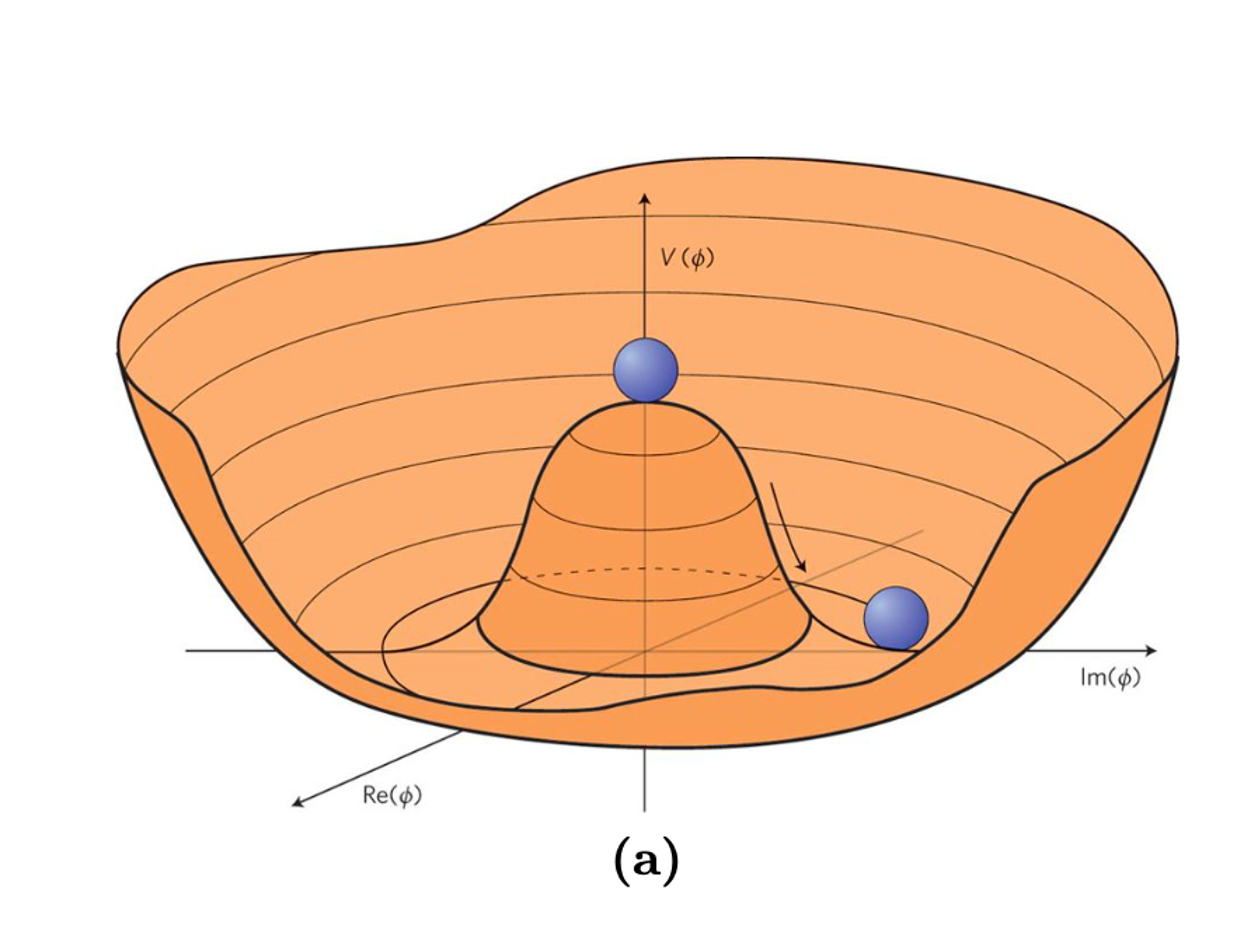
\includegraphics[width=0.7\textwidth,clip]{figures/Chapter1/MexHat.png}
    \end{center}
    \caption["墨西哥帽"势能示意图]{"墨西哥帽"势能示意图}
    \label{fig:MexHat}
\end{figure}

手征对称性的破缺也导致了真空中的夸克凝聚(quark condense)。可以从$\pi$介子的质量和夸克凝聚的关系(Gell-Mann-Oakes-Renner关系)中得到:

\begin{equation}
    m_{\pi}^2 f_{\pi}^2 = -2\bar{m}\langle 0|\bar{q}q|0 \rangle
\end{equation}
其中$\bar{m} \approx 6~ {\rm MeV/c^2} $是u和d夸克的平均质量。从这个关系式中我们可以看到真空中的夸克凝聚的值$\langle 0|\bar{q}q|0 \rangle \approx (-250 {\rm~MeV})^3$。这也是手征对称性破坏的标志之一。

在实验上对手征对称恢复的观测可以通过测量手征多重态的质量分布来做到,例如$\rho^0(770)$和$a_1(1260)$。如果没有手征对称性破缺这两个态将会是简并的,然而在实验的测量中却发现他们两个的质量差别很大:$m_{\rho^0} \approx 770 ~{\rm MeV/c^2}$, $m_{a_1} \approx 1260 ~{\rm MeV/c^2}$。这种质量的差别不能简单的被u夸克和d夸克的质量差别来描述,很可能由手征对称性的破缺带来。

人们预期这种夸克凝聚态会在高温($T > T_c^{chiral}$)、高密($n > n_c^{chiral}$)的条件下发生改变。因此人们期待在这种条件下可以看到从带有自发手征对称性破缺强子物质态到手征恢复的物质态的转变。但需要注意的是手征恢复的的相变条件和量子色动力学物质解禁闭的相变条件并不相同,人们预期手征对称恢复的相变温度要高于夸克胶子等离子体的相变温度,即在相同的重子势下,$T_c^{chiral} > T_c^{QGP}$。这就意味着夸克胶子等离子体可能在手征对称恢复没有达到的情况下存在,同时也意味着存在手征对称恢复的时候夸克和胶子一定是解禁闭的。在实验上手征对称恢复一个很重要的观测量便是$\rho^0$和$a_1$质量的简并,对他们质量谱的测量是我们直接对手征对称恢复进行观测的一个很重要的手段。
